\documentclass{../source/zjureport}

\major{信息工程}
\name{周灿松}
\title{实验设计报告}
\stuid{3190105055}
\college{信息与电子工程学院}
\date{\today}
\lab{教7-108}
\course{计算机组成与设计}
\instructor{刘鹏}
\grades{}
\expname{Cache Controller}
\exptype{代码编写}
\partner{无}

\begin{document}
    \makecover
    \tableofcontents
    \newpage
    \section{有限状态机设计}
        \subsection{状态编码设计}
            如图\ref{state diagram}所示,我参考教材5.9节设计了一共四个状态,分别是:空闲状态IDLE,Tag位比较状态CompareTag,写回状态WriteBack以及分配状态Allocate,各个状态作用如下
            \begin{enumerate}
                \item IDLE:等待来自CPU的控制信号ld以及st,当这两个信号有效时,转移到CompareTag状态。
                \item CompareTag:比较来自Cache的对应Block的Tag位与来自CPU的地址Addr的[31:11]位,同时根据对应Block的Valid与Dirty位判断是Hit或者Miss,以及转移到对应的状态。
                \item WriteBack:在此状态将Cache中的Block写回L2 Cache中,当接收到来自L2的写回完成信号write_done后,写回完成,状态转移到Allocate。
                \item Allocate:此状态用于在L1 Cache miss时将L2 Cache中的值加载到L1 Cache中,当得到写入完成信号l2_ack后,说明写入完成,状态切换到CompareTag。
            \end{enumerate}

            \begin{figure}[H]
                \centering
                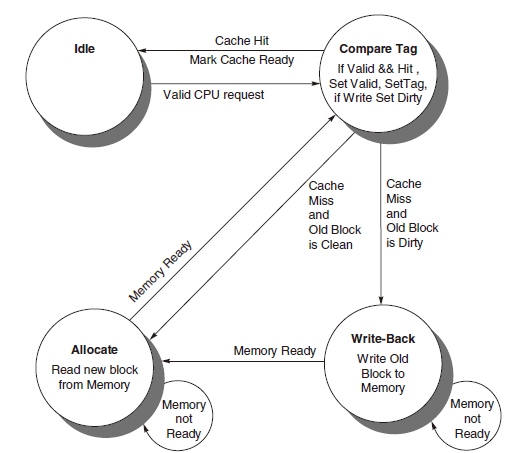
\includegraphics[]{figure/fourState.png}
                \caption{state diagram}
                \label{state diagram}
            \end{figure}

            各个状态的状态编码如表\ref{状态编码}所示

            \begin{table}[H]
                \centering
                \begin{tabular}{|c|c|}
                \hline
                \multicolumn{2}{|c|}{\textbf{状态编码}} \\ \hline
                IDLE                 & 00           \\\hline
                CompareTag           & 01           \\\hline
                WriteBack            & 10           \\\hline
                Allocate             & 11          \\\hline
                \end{tabular}
                \caption{状态编码}
                \label{状态编码}
            \end{table}

        \subsection{状态转换表}
        状态转移表如表\ref{状态转移表}所示,‘--’表示在当前状态转移情况下不关心该信号。
        \begin{table}[H]
            \begin{tabular}{|c|c|c|c|c|c|c|c|c|}
            \hline
            \textit{\textbf{state}}     & \textbf{ld} & \textbf{st} & \textbf{tag==addr{[}31:11{]}} & \textbf{dirty} & \textbf{valid} & \textbf{l2\_ack} & \textbf{write\_done} & \textbf{nextstate}          \\ \hline
            \multirow{4}{*}{IDLE}       & 0           & 0           & --                            & --             & --             & --               & --                   & IDLE                        \\ \cline{2-9} 
                                        & 0           & 1           & --                            & --             & --             & --               & --                   & \multirow{3}{*}{CompareTag} \\ \cline{2-8}
                                        & 1           & 0           & --                            & --             & --             & --               & --                   &                             \\ \cline{2-8}
                                        & 1           & 1           & --                            & --             & --             & --               & --                   &                             \\ \hline
            \multirow{3}{*}{CompareTag} & --          & --          & --                            & 0              & 0              & --               & --                   & Allocate                    \\ \cline{2-9} 
                                        & --          & --          & --                            & 1              & 0              & --               & --                   & WriteBack                   \\ \cline{2-9} 
                                        & --          & --          & --                            & --             & 1              & --               & --                   & IDLE                        \\ \hline
            \multirow{2}{*}{WriteBack}  & --          & --          & --                            & --             & --             & --               & 1                    & Allocate                    \\ \cline{2-9} 
                                        & --          & --          & --                            & --             & --             & --               & 0                    & WriteBack                   \\ \hline
            \multirow{2}{*}{Allocate}   & --          & --          & --                            & --             & --             & 1                & --                   & CompareTag                  \\ \cline{2-9} 
                                        & --          & --          & --                            & --             & --             & 0                & --                   & Allocate                    \\ \hline
            \end{tabular}
            \caption{状态转移表}
            \label{状态转移表}
            \end{table}
        \subsection{FSM图}
        FSM图如图\ref{FSM}所示。
        \begin{figure}[H]
            \centering
            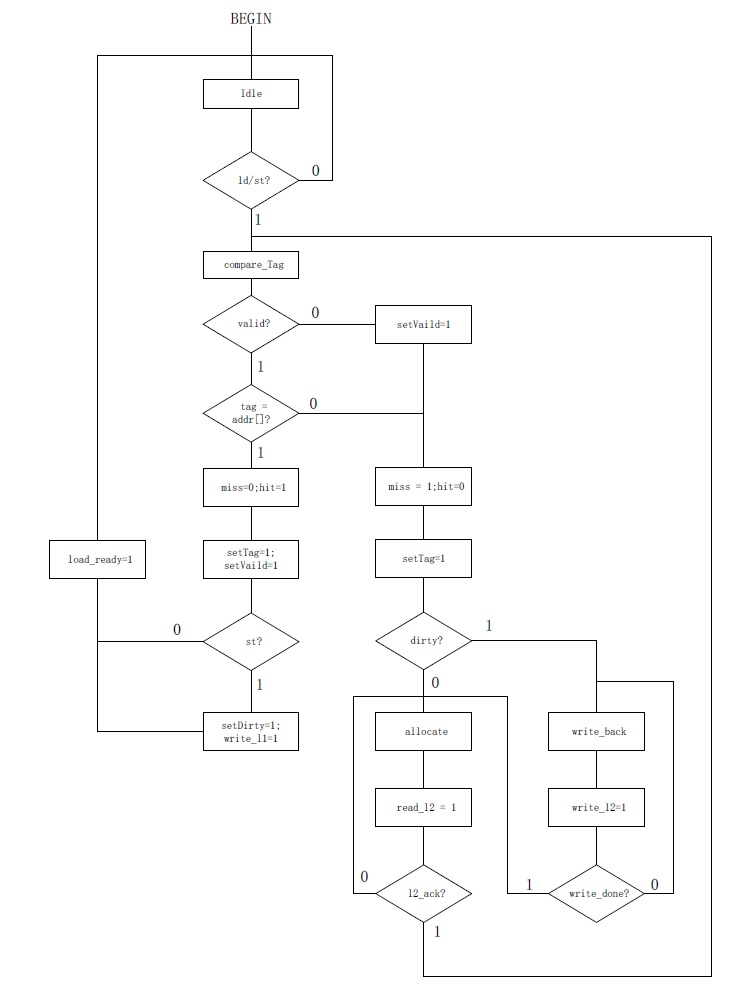
\includegraphics[scale = 0.6]{figure/FSM.png}
            \caption{FSM图}
            \label{FSM}
        \end{figure}
    \section{电路设计}
        我通过Vivado软件进行了电路设计,电路图如图\ref{电路图}所示。
        \begin{figure}[H]
            \centering
            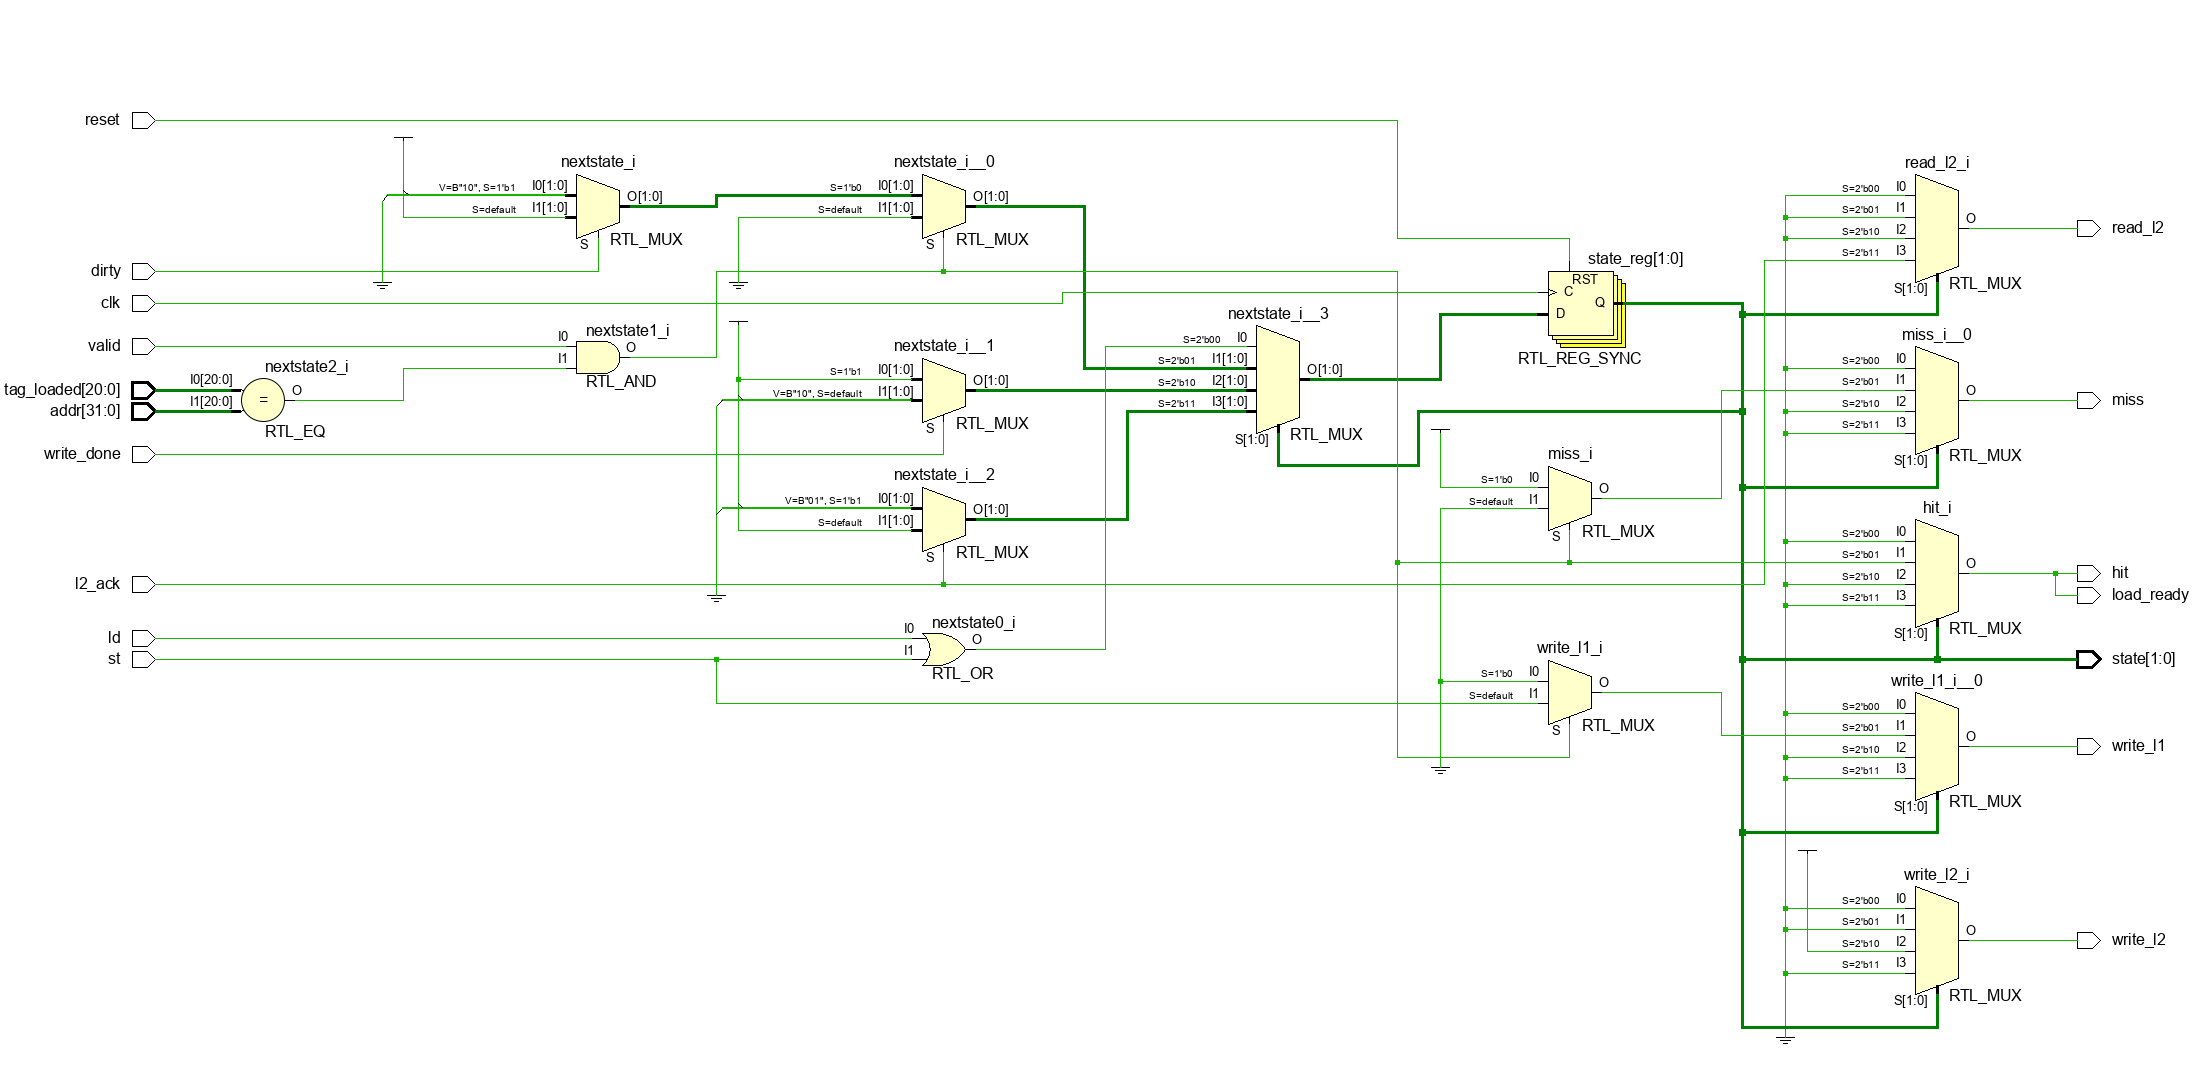
\includegraphics[width = \textwidth]{figure/电路图.png}
            \caption{电路图}
            \label{电路图}
        \end{figure}

    \section{Verilog实现}
        \subsection{信号含义详细阐释}
        \begin{enumerate}
            \item clk:时钟信号
            \item reset:重置信号
            \item ld:数据由L1加载到CPU
            \item st:数据由CPU写入L1
            \item addr:数据所在地址
            \item valid:L1的有效位
            \item dirty:L1的脏位
            \item tag_loaded:L1对应位置的Tag
            \item l2_ack:数据是否完成从L2写入L1的过程
            \item write_done:数据是否完成从L1写回buffer的过程
            \item hit:hit信号
            \item miss:miss信号
            \item load_ready:L1数据是否准备就绪
            \item write_l1:使能L1的写入功能
            \item read_l2:发向L2的load指令
            \item write_l2:使能L1写回buffer
        \end{enumerate}
        \subsection{Verilog代码}
            Cache控制器的代码Listing \ref{cache}所示。
            
        \subsection{测试样例}
            所用测试代码如Listing \ref{test}所示。
            
        \subsection{测试结果}
            Cache Controller测试结果如图\ref{结果}所示,各个控制信号正确,功能能够正常实现
            \begin{figure}[H]
                \centering
                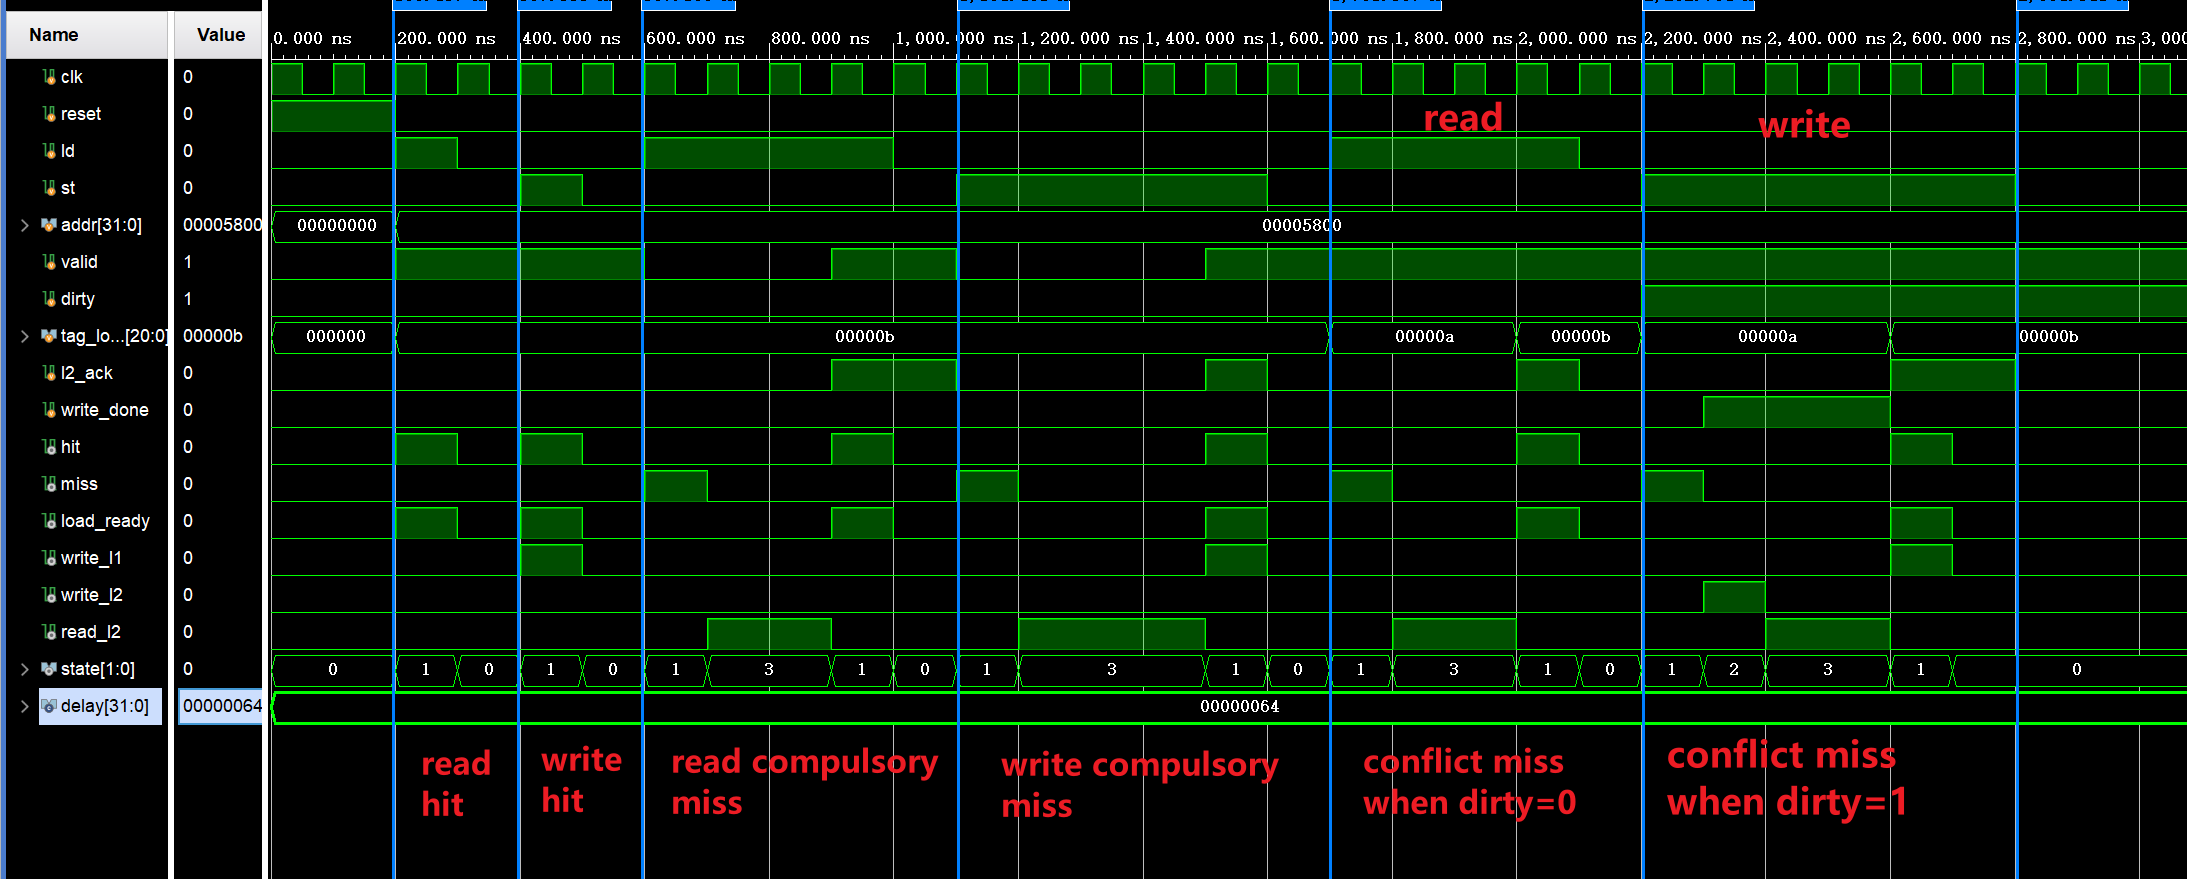
\includegraphics[width = \textwidth]{figure/测试.png}
                \caption{测试结果}
                \label{结果}
            \end{figure}
    \section{心得体会}
        通过本次实验,我对Cache的整个控制机制有了一个更加具体的理解,同时也补足了自己在学习Cache相关内容时所遗漏的知识点。

        除此之外,这次实验也是我第一次编写testbench文件,对于Verilog语言的测试方式有了一个更加透彻的掌握。

    \section{附录}
        \subsection{cache代码}
        \lstinputlisting[
            language = Verilog,
            caption = Cache控制器代码,
            label = cache
        ]{code/cache_controller.v}
        \subsection{测试代码}
        \lstinputlisting[
            language = Verilog,
            caption = Cache控制器测试文件,
            label = test
        ]{code/test_tb.v}
\end{document}